\section{MÔ HÌNH HỆ THỐNG}
\subsection{Các linh kiện phần cứng}
Trong mô hình khảo sát, chúng ta xét một hệ thống thu thập số liệu đa chiều sử dụng mạch xử lý trung tâm là ESP8266. Để tăng cường chất lượng phát hiện sự cố, tổ hợp ba cảm biến sau được sử dụng:

\begin{itemize}
    \item \textbf{Cảm biến nhiệt độ DHT22}: Dữ liệu nhiệt độ (ký hiệu là $t$) được đo liên tục để phát hiện sự gia tăng nhiệt độ vượt ngưỡng báo động được thiết lập là $TEMP\_THRESHOLD = 20.0^\circ\text{C}$.
    
    \begin{figure}[H]
    \centerline{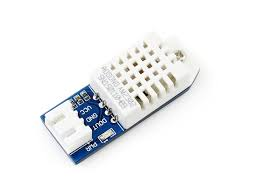
\includegraphics[width=0.45\linewidth]{figures/dht22.jpg}}
    \caption{Cảm biến nhiệt độ DHT22.}
    \label{fig:dht22}
    \end{figure}

    \item \textbf{Cảm biến MQ2}: Chịu trách nhiệm đo nồng độ các loại khí dễ cháy. Tín hiệu đầu vào $gasValue$ được lấy qua bộ chuyển đổi ADC và so sánh với ngưỡng an toàn $GAS\_THRESHOLD = 500$.
    
    \begin{figure}[H]
    \centerline{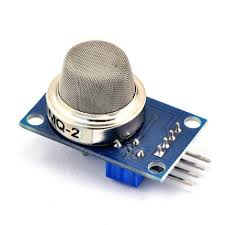
\includegraphics[width=0.45\linewidth]{figures/mq2.jpg}}
    \caption{Cảm biến khí gas MQ2.}
    \label{fig:mq2}
    \end{figure}

    \item \textbf{Cảm biến phát hiện ngọn lửa}: Đưa ra tín hiệu dạng logic (mức LOW khi phát hiện có ngọn lửa) để xác nhận có hỏa hoạn xảy ra.
    
    \begin{figure}[H]
    \centerline{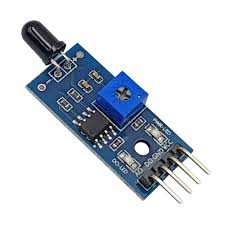
\includegraphics[width=0.45\linewidth]{figures/flame_sensor.jpg}}
    \caption{Cảm biến phát hiện ngọn lửa.}
    \label{fig:flame}
    \end{figure}
\end{itemize}

Về cơ chế xử lý, đầu tiên, xét sự truyền tín hiệu và phản hồi với các bộ chấp hành, chúng ta có thể mô tả hệ thống hoạt động thông qua các ngoại vi sau:

\begin{itemize}
    \item \textbf{Động cơ Servo}: Điều khiển mở cửa sổ (quay $90^\circ$) để thông gió và tạo khoảng không thoát khí.
    
    \begin{figure}[H]
    \centerline{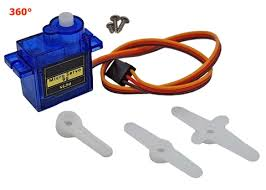
\includegraphics[width=0.45\linewidth]{figures/servo.jpg}}
    \caption{Động cơ Servo.}
    \label{fig:servo}
    \end{figure}

    \item \textbf{Relay (Rơ-le)}: Đóng cắt nguồn điện cho quạt hút, giúp đẩy không khí độc ra khỏi hiện trường.
    
    \begin{figure}[H]
    \centerline{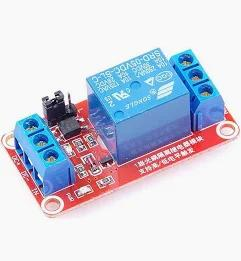
\includegraphics[width=0.45\linewidth]{figures/relay.jpg}}
    \caption{Module Relay.}
    \label{fig:relay}
    \end{figure}

    \item \textbf{Còi báo động (Buzzer)}: Phát âm thanh cảnh báo cường độ cao tại chỗ.
    
    \begin{figure}[H]
    \centerline{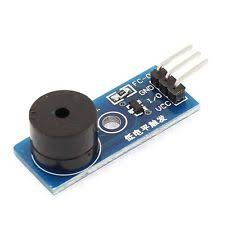
\includegraphics[width=0.45\linewidth]{figures/buzzer.jpg}}
    \caption{Còi báo động (Buzzer).}
    \label{fig:buzzer}
    \end{figure}

    \item \textbf{Đèn LED RGB}: Thay đổi màu sắc (Xanh lá, Vàng, Đỏ) để thông báo mức độ khẩn cấp một cách trực quan.
    
    \begin{figure}[H]
    \centerline{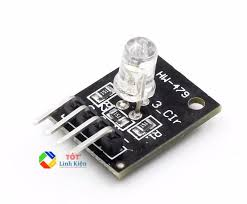
\includegraphics[width=0.45\linewidth]{figures/module_led.jpg}}
    \caption{Module Đèn LED RGB.}
    \label{fig:led}
    \end{figure}
\end{itemize}

Chú ý rằng: toàn bộ hệ thống hoạt động lặp liên tục, chu kỳ lấy mẫu được ấn định là 2000 mili-giây.


\begin{figure*}[!ht]
\centering
\begin{tikzpicture}[
    node distance=1.5cm and 2.5cm,
    sensor/.style={draw, rectangle, minimum width=2.5cm, minimum height=1cm, align=center, fill=blue!10},
    mcu/.style={draw, rectangle, minimum width=3cm, minimum height=6.5cm, align=center, fill=green!10, rounded corners},
    actuator/.style={draw, rectangle, minimum width=2.5cm, minimum height=1cm, align=center, fill=red!10},
    cloud/.style={draw, ellipse, minimum width=3cm, minimum height=1.5cm, align=center, fill=cyan!10},
    arrow/.style={-stealth, thick}
]

% Khối MCU
\node[mcu] (esp) {ESP8266};

% Khối cảm biến (Bên trái)
\node[sensor, left=2cm of esp] (mq2) {Cảm biến \\ MQ2};
\node[sensor, above=0.5cm of mq2] (dht) {Cảm biến \\ DHT22};
\node[sensor, below=0.5cm of mq2] (flame) {Cảm biến \\ Ngọn lửa};

% Khối chấp hành (Bên phải)
\node[actuator, right=2cm of esp, yshift=0.75cm] (relay) {Relay \\ (Quạt hút)};
\node[actuator, above=0.5cm of relay] (servo) {Động cơ \\ Servo};
\node[actuator, right=2cm of esp, yshift=-0.75cm] (buzzer) {Còi báo động};
\node[actuator, below=0.5cm of buzzer] (led) {Đèn LED \\ RGB};

% Khối Cloud (Bên dưới)
\node[cloud, below=1cm of esp] (blynk) {Blynk App};

% Vẽ các mũi tên
\draw[arrow] (dht.east) -- (dht.east -| esp.west);
\draw[arrow] (mq2.east) -- (esp.west);
\draw[arrow] (flame.east) -- (flame.east -| esp.west);

\draw[arrow] (esp.east |- servo.west) -- (servo.west);
\draw[arrow] (esp.east |- relay.west) -- (relay.west);
\draw[arrow] (esp.east |- buzzer.west) -- (buzzer.west);
\draw[arrow] (esp.east |- led.west) -- (led.west);

\draw[arrow, <->] (esp.south) -- (blynk.north) node[midway, right] {WiFi};

\end{tikzpicture}
\caption{Sơ đồ khối của hệ thống.}
\label{fig:block_diagram}
\end{figure*}

\subsection{Sơ đồ khối và mô tả hoạt động}

Sơ đồ khối hệ thống (Hình \ref{fig:block_diagram}) bao gồm 4 thành phần chính:
\begin{itemize}
    \item \textbf{Khối đầu vào (Cảm biến)}: Gồm cảm biến nhiệt độ DHT22, cảm biến khí gas MQ2 và cảm biến ngọn lửa. Các cảm biến này liên tục thu thập dữ liệu môi trường để gửi về vi điều khiển xử lý.
    \item \textbf{Khối xử lý trung tâm}: Sử dụng vi điều khiển ESP8266 làm bộ não của hệ thống. Khối này đọc dữ liệu từ các cảm biến với chu kỳ lặp lại, phân tích và so sánh với các ngưỡng an toàn để đưa ra quyết định xử lý, đồng thời gửi dữ liệu lên ứng dụng qua WiFi.
    \item \textbf{Khối đầu ra (Chấp hành)}: Dựa trên tín hiệu điều khiển từ ESP8266, khối đầu ra thực hiện các hành động: Động cơ Servo điều khiển mở cửa sổ, Relay đóng mạch bật quạt hút khí, Còi báo động (Buzzer) phát âm thanh, và Đèn LED RGB đổi màu tương ứng với các cấp độ cảnh báo.
    \item \textbf{Khối giám sát từ xa}: ESP8266 kết nối WiFi để truyền dữ liệu lên ứng dụng Blynk. Người dùng có thể theo dõi trực tiếp các thông số môi trường, trạng thái của hệ thống và nhận thông báo khẩn cấp từ xa.
\end{itemize}

\subsubsection{Bảng kết nối phần cứng}
Dựa trên sơ đồ khối và chức năng đã đề cập, toàn bộ các linh kiện trong hệ thống được kết nối với vi điều khiển trung tâm ESP8266 (board NodeMCU) thông qua cấu hình các chân tín hiệu (pin mapping) được liệt kê chi tiết trong Bảng \ref{tab:input_pins} và Bảng \ref{tab:output_pins}.

\begin{table}[H]
\caption{Kết nối khối cảm biến với ESP8266.}
\label{tab:input_pins}
\centering
\renewcommand{\arraystretch}{1.3}
\resizebox{\columnwidth}{!}{%
\begin{tabular}{|c|p{4cm}|c|c|}
\hline
\textbf{STT} & \textbf{Linh kiện / Thiết bị} & \textbf{Chân ESP8266} & \textbf{Chân trên NodeMCU} \\
\hline
1 & Cảm biến nhiệt độ DHT22 & GPIO 4 & D2 \\
\hline
2 & Cảm biến khí gas MQ2 & ADC0 & A0 \\
\hline
3 & Cảm biến phát hiện ngọn lửa & GPIO 5 & D1 \\
\hline
\end{tabular}%
}
\end{table}

\begin{table}[H]
\caption{Kết nối khối chấp hành với ESP8266.}
\label{tab:output_pins}
\centering
\renewcommand{\arraystretch}{1.3}
\resizebox{\columnwidth}{!}{%
\begin{tabular}{|c|p{4cm}|c|c|}
\hline
\textbf{STT} & \textbf{Linh kiện / Thiết bị} & \textbf{Chân ESP8266} & \textbf{Chân trên NodeMCU} \\
\hline
1 & Động cơ Servo & GPIO 2 & D4 \\
\hline
2 & Module Relay (Quạt hút) & GPIO 15 & D8 \\
\hline
3 & Còi báo động (Buzzer) & GPIO 0 & D3 \\
\hline
4 & Đèn LED RGB (Chân Đỏ - R) & GPIO 14 & D5 \\
\hline
5 & Đèn LED RGB (Chân Xanh lá - G) & GPIO 12 & D6 \\
\hline
6 & Đèn LED RGB (Chân Xanh dương - B) & GPIO 13 & D7 \\
\hline
\end{tabular}%
}
\end{table}

\subsection{Thực hiện hệ thống}
Dựa trên thiết kế lý thuyết và sơ đồ kết nối, mô hình hệ thống giám sát và cảnh báo thông minh đã được lắp ráp và triển khai thực tế. Hình \ref{fig:real_system} thể hiện toàn cảnh phần cứng của hệ thống sau khi hoàn thiện, với đầy đủ các cảm biến và cơ cấu chấp hành được kết nối tới vi điều khiển trung tâm ESP8266. 

\begin{figure}[H]
\centerline{%
  \begin{tikzpicture}
    \draw[dashed, thick, fill=gray!10] (0,0) rectangle (0.8\columnwidth, 4cm);
    \node[align=center] at (0.4\columnwidth, 2cm) {\bfseries [Ảnh thực tế sẽ chèn vào đây]};
  \end{tikzpicture}%
}
% GHI CHÚ: Khi bạn đã chụp ảnh thực tế, hãy XÓA khối tikzpicture phía trên 
% và BỎ COMMENT dòng dưới đây (thay bằng tên file ảnh của bạn):
% \centerline{\includegraphics[width=0.7\linewidth]{figures/ten_file_anh.jpg}}
\caption{Hình ảnh thực tế của hệ thống (Sẽ cập nhật ảnh thực tế sau).}
\label{fig:real_system}
\end{figure}

Trong quá trình triển khai, các linh kiện được bố trí khoa học, đảm bảo kết nối vật lý chắc chắn. Các cảm biến DHT22, MQ2 và cảm biến ngọn lửa được đặt ở các vị trí dễ dàng phát hiện các thay đổi bất thường của môi trường. Các thiết bị chấp hành như động cơ Servo, quạt hút, module LED và còi báo cũng được lắp đặt hợp lý để phản ứng ngay lập tức khi nhận được tín hiệu cảnh báo từ hệ thống.
